% TODO:
%   - References in section helping people with disabilities for examples
%   - Refs to sections check if truly explained there
%   - Cleanup of text
%   - Longer more descriptive titles
%   - Invasive is ECoG instead of EEG?
%   - Specify better what a BCI is in the first sentences
% ----------  
% Questions:
%   -

%  Today, amplifiers exist that are built in the electrode cap and are so resistant to movement artefacts that data collection in the field is no longer a critical issue.
% SOURCE: bci_history

% Wolpaw defines the “perfect” BCI as a safe and affordable system which works all the time, does not require the permanent assistance of a technician or a scientist, restores communication at “normal” speed, is aesthetically acceptable, is reliable and, for the same function, does not require more concentration for a patient user than what it does for an able-bodied person [1]. Despite recent development aimed at improving the current state of BCI systems, there are still several challenges that must be overcome before building an usable and effective BCI, like for example, the high cost associated with the required EEG recording system
% SOURCE: cheap_bci_feasibility

% Uncomment this if the use of parts is desired
%\part{First part}


% In a new chapter, reset the GLS to once again use the full version in the first occurrence
\glsresetall

\chapter{Brain-Computer interfaces}
\label{ch:bci}

% ---------------------------------------------- 

\section{Introduction to BCIs}
\label{sec:bci_introduction}

\Glspl{bci} and \glspl{bmi} are starting to gather more interest from the general public.
These systems, consisting of hardware and software, aim to read and stimulate a user's brain signals for a wide range of applications.
Neuralink, an Elon Musk company, helped to popularize them outside of the research field.
Neuralink's initial white paper discusses its aim to create a scalable high-bandwidth \gls{bmi} system, focusing on its mechanical achievements \citep{neuralink_whitepaper}.
Only a mere year later, the company held a conference with a live demo of their \gls{bmi} implanted into the skulls of pigs.

Whilst such novel interaction applications have yet to see widespread market adoption, \glspl{bci} have been studied for decennia by researchers such as \citet{early_bci}.
An in-depth history from \glspl{bci} can be found from Andrea \citet{bci_history}.
\citet{bci_review} gives an overview of the different kinds of \glspl{bci} and corresponding techniques to be used.
These sources give a great high-level insight into the technology and terminology used in this field.
A good introductory book on \glspl{bci} from this same period is one from the well-known Professor in this field: Jonathan Wolpaw \citep{bci_book}.

Whilst the main components used today remain relatively similar to those discussed in these older sources, the hardware complexity and model capabilities has been evolving drastically.
An important issue researchers keep getting confronted with is the fact that there are still a lot of mysteries about the brain's inner workings, leaving many of the finer intercepted brain signals unexplained.
\citet{brainmapping} states that the progress of mapping the brain and its billions of sensors and connections is accelerating yet still far from finished.
This mapping would be a huge step in understanding the brain.

Luckily, novel \gls{ml} techniques can help with processing and reasoning on the data these systems collect.
Especially due to recent developments in \gls{dl} and \gls{nn}, \glspl{bci} are being used more in treating neurological diseases \citep{bci_diseases} but also more commercial applications, like a brain-monitoring meditation aids as discussed by \citet{interaxon_tests}.

A challenge with \gls{dl} applications in general, and certainly with \glspl{bci}, is the fact that training a deep learner in both a supervised and unsupervised manner can take a lot of data and time and be unpredictable due to its black-box principle.
These things are unwished-for in \gls{bci} systems, especially when not only reading but also stimulating brain signals.
In general, full supervised learning isn't possible either due to the lack of understanding of the brain signals.
Therefore, low-confidence labelled data is often used in a semi-supervised fashion as explained by \citet{deep_learn_low_label}.

% ---------------------------------------------- 

\section{Growing scientific and commercial interest in BCIs}
\label{sec:bci_gaining_popularity}

As was already discussed, Neuralink, a company by Elon Musk aiming to provide an invasive \gls{bci} to be used by the masses as a means for fast communication between humans and machines, has put the research field in a new daylight.
However, the reason \gls{bci} applications are gaining more and more interest follows from a wide variety of reasons.
The following section will discuss the most important ones.

% - - - - - - - - - -

\subsection{New funding sources for BCI related research}
\label{subsec:bci_gaining_popularity_big_tech}
Big tech has been catching on with the possibilities \glspl{bci} bring, and the amount of money they can earn from it.
Their goals lie far from the long medical history of the field, although profitability is an important factor in most medical applications as well.
Besides Neuralink, companies like Meta, Valve, Neurable, InteraXon and many more are exploring the commercial possibilities of \glspl{bci} as well, both through funding or internal research \citep{facebook_bci_keyboard, valve_bci_interest, neurable_white_paper, interaxon_tests}.
There seem to be two main focuses of the technology in the commercial space.
Using the new interaction method to perform work more efficiently and using it for recreational purposes.

Meta, formerly known as Facebook, has publicly announced it had provided funds for research on the use of a \gls{bci}-system to restore speech functionalities for people suffering from anarthria \citep{facebook_bci_keyboard, facebook_bci_blog}.
\Citet{facebook_bci_keyboard} achieved an average of 15 words per minute through a highly specialized and non-mobile system, decoded with a median error of 25\%.
The setup is shown in Figure \ref{fig:intro_medical_vs_commercial_1}.
\Citet{facebook_bci_keyboard} described it as way of giving a voice to people with speech impairment.
However, it is not hard to imagine the commercial interest of Meta in developing a more general \textit{virtual keyboard} to enable fast \textit{thought to speech} applications usable by the masses.
Such a virtual keyboard could replace certain speech-to-text applications already broadly used for commercial purposes.
With this broader application in mind, the work by \citet{facebook_bci_keyboard} becomes even more interesting as it doesn't rely on \glspl{erp} that requires explicit stimulation.
The latter is required by most other virtual keyboard attempts as discussed by \citet{bci_keyboard}.
In the same blog post by \citet{facebook_bci_blog}, it is also mentioned that Meta has interest in using \glspl{bci} for high-bandwidth interactions in AR/VR.
However, Meta has been subject to multiple privacy concerns lately \citep{facebook_drama1, facebook_drama2}.
The company's reputation has been damaged from this which doesn't help in selling the concept of them having a \gls{bci} which allows them to read the brain activity of the users.
This could explain why they have recently started to shift their focus from \glspl{bci} towards muscle-based interfaces using \gls{emg} \citep{facebook_bci_blog}.

For recreational use, \glspl{bci} have been found in commercial products already.
The headsets by InteraXon, produced under the Muse brand, are one of the earliest examples, with their first version being released in 2014.
The first iteration of this product was advertised as a meditation aid.
This headset relies on measuring Theta waves in the brain, which are lower frequency waves that suggest a user is meditating.
The actual accuracy and usefulness of the system are debated, as discussed by \citet{interaxon_tests}.
However, InteraXon, the company behind the Muse headset, plays an important role in the commercialisation of \glspl{bci} as they have made cheaper and more visually attractive systems available in the open market.
Section \ref{subsec:bci_gaining_popularity_better_processing} will go into further detail on this.
A more recent version of the headband, named Muse 2, also aids in sleep monitoring.
Muse 2 is shown in Figure \ref{fig:intro_medical_vs_commercial_2}.

% TODO: citing for sources of img?
\begin{figure}[ht]
  \begin{minipage}{\textwidth}
    \centering
    \begin{subfigure}{.48\textwidth}
        \centering
        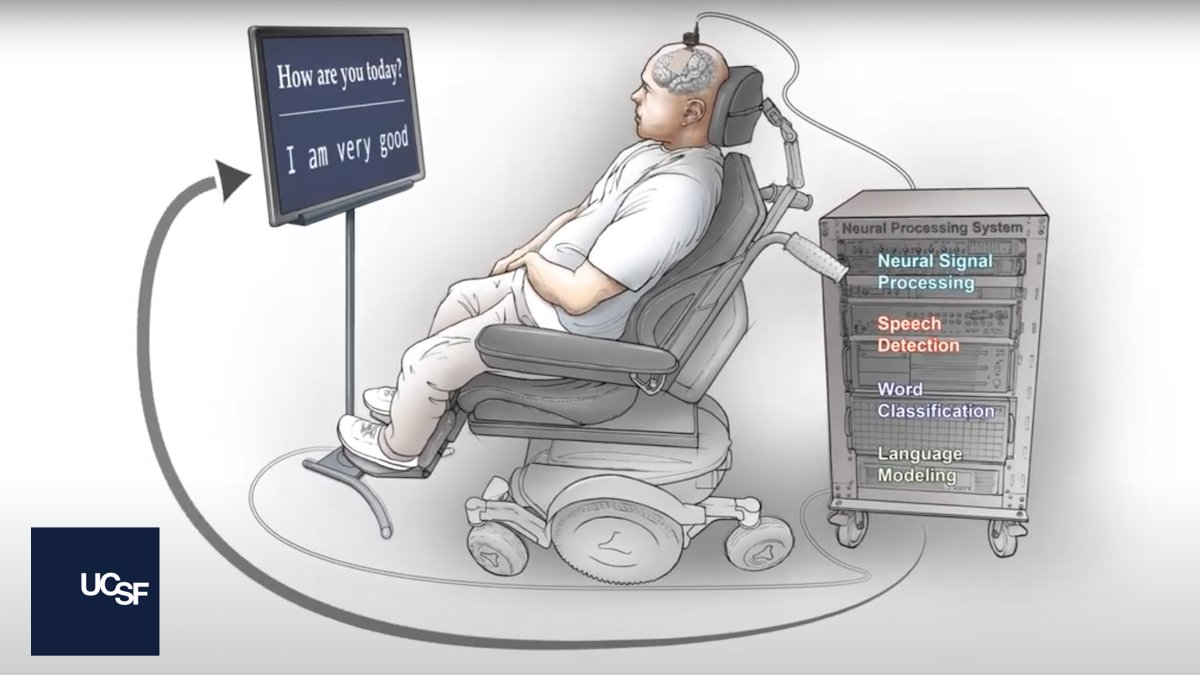
\includegraphics[width=\textwidth]{images/introduction/fb_bci_keyboard.jpg}
        \captionsetup{width=0.9\linewidth}
        \captionsetup{justification=centering}
        \caption{\gls{bci}-system to restore speech functionalities for people suffering from anarthria. Setup and illustration by \citet{facebook_bci_keyboard}.}
        \label{fig:intro_medical_vs_commercial_1}
    \end{subfigure}
    \hfill
    \begin{subfigure}{.48\textwidth}
        \centering
        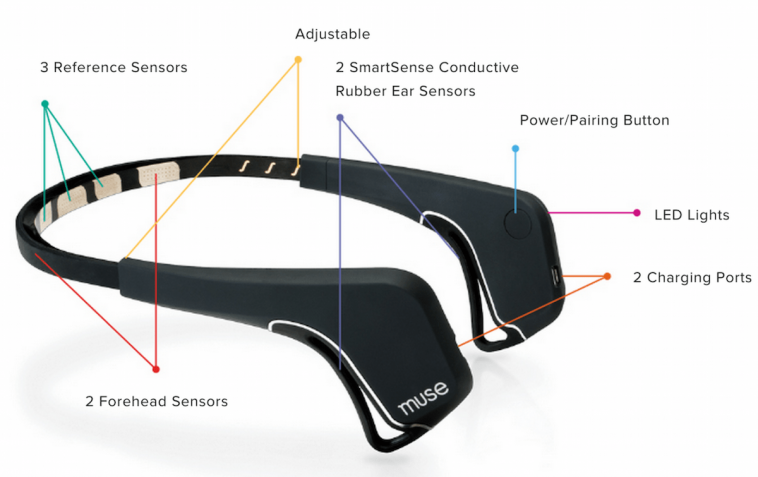
\includegraphics[width=\textwidth]{images/introduction/muse.png}
        \captionsetup{width=0.9\linewidth}
        \captionsetup{justification=centering}
        \caption{Commercial \gls{bci}-system sold as meditation and sleep tracking aid. Product and illustration by Muse\footnotemark[1].}
        \label{fig:intro_medical_vs_commercial_2}
    \end{subfigure}
    \captionsetup{width=0.9\linewidth}
    \captionsetup{justification=centering}
    \caption{Contrast between a complex and bulky medical-grade \gls{bci}-system and a simpler and portable commercial \gls{bci} application.}
    \footnotetext[1]{\url{https://choosemuse.com/muse-2/}}
    \label{fig:intro_medical_vs_commercial}
  \end{minipage}  
\end{figure}

Perhaps the most prominent short term coming commercial use of \glspl{bci} is in combination with \gls{vr} and \gls{ar}.
Besides \citet{facebook_bci_blog}, Valve, has also said it is actively researching how to use \glspl{bci} as input in \gls{vr} games \citep{valve_bci_interest}.
Valve is the company behind Steam, one of the world's largest game marketplaces.
To achieve this, Valve (specialized in gaming), OpenBCI (specialized in \gls{bci} hardware and software) and Tobii (specialized in eye-tracking) are working together to develop both open-source hardware and software \citep{bci_valve}.

Another stream of money is coming from the military, as the U.S. Department of Defense and others have shown interest in a wide variety of applications using \glspl{bci} \citep{bci_military}.
All of these big companies and organisations with a lot of financial support are bound to accelerate the development of more general use \gls{bci}-systems.
Figure \ref{fig:bci_money} shows the funding of \gls{bci}-related companies founded after 2010 as a rough indication of how much money is spent on start-up companies in the field.

\begin{figure}[ht]
    \centering
    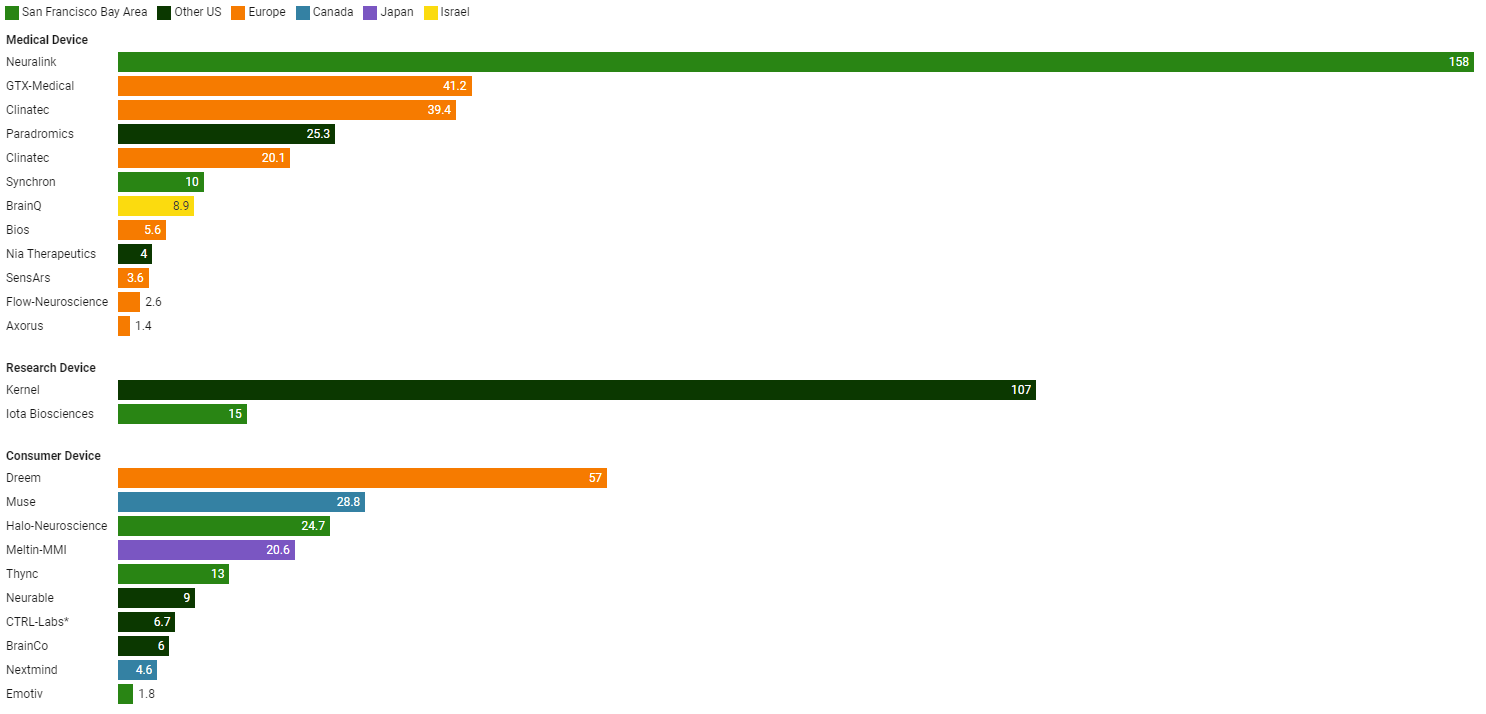
\includegraphics[width=\linewidth]{images/introduction/bci_money.png}
    \captionsetup{width=0.9\linewidth}
    \captionsetup{justification=centering}
    \caption{Funding of newer \gls{bci} related companies depicted in millions (USD).\\Figure by \citet{bci_money} based on data by Meta from 2019. It is noted that only a selected portion of companies is shown that were created after 2010. Older companies with exponentially higher funding exist.}
    \label{fig:bci_money}
\end{figure}

% - - - - - - - - - -

\subsection{Improved brain-signal measuring facilities}
\label{subsec:bci_gaining_popularity_better_measuring}

Most \glspl{bci} rely on \gls{eeg} as source of data and this paper will focus mainly on \gls{eeg} driven \gls{bci}.
Chapter \ref{ch:biomedical_signals} goes into depth on what \gls{eeg} is, the equipment used and more.
For this introduction, it suffices to know that \gls{eeg} measures the electrical potential difference, in \gls{mv}, between electrodes placed inside or on the skull.

As discussed further in section \ref{subsec:biomedical_signals_measuring_equipment}, wet electrodes are widely considered to produce better data quality then dry electrodes in their current form \citep{wet_vs_dry, dry_electrode_status, wet_dry_comparison_experiment}.
However, wet electrodes make use of a gel that is not only time consuming to apply but also cosmetically inconvenient, both of which are bad properties for a (commercial) \gls{bci}.
The gel could also cause allergic effects for the user and artefacts in measurements due to a change in viscosity of the gel over time.
Luckily, the advancements in both active-electrode amplification and dry electrodes are making the gap with wet electrodes smaller and smaller \citep{wet_vs_dry, dry_electrode_status, wet_dry_comparison_experiment}.
Dry electrodes don't require the application of a gel and due to the active-electrode amplification, they can be used in more challenging environments outside of the lab \citep{wet_vs_dry}.
These benefits of dry electrodes with usable data quality make real-world applications and commercialisation of \glspl{bci} more viable.

However, an issue that remains, even with the best active wet electrodes, is the contrast between spatial and temporal resolution.
\gls{eeg} is known to have a good temporal resolution but rather poor spatial resolution.
A good spatial resolution would mean that the measurement from electrodes corresponds only to a small, known region of the brain, typically underneath that electrode.
Such a correlation is helpful as it reduces noise and increases interpretability.
It also allows for fewer electrodes to be used if only the activity of certain areas of the brain is of interest.
However, improving spatial resolution has been proven challenging \citep{spatial_resolution}.
Besides poor signal-to-noise ratios of the measurements, this is also caused by the anatomy of the brain.
Different structures, such as the skull and \gls{csf}, \textit{blur} and \textit{disperse} the perceived signal, making it hard to track where the measured signal came from.
Whilst increasing the number of electrodes placed on the skull already physically limits the region under a signal electrode, it makes electrodes more prone to overlap from signals also measured by other electrodes.
Because of this, simply adding electrodes only improves the spatial resolution to a certain point.
Besides this, there is also the issue that decreasing the distance between electrodes introduces the need for placing more electrodes to cover the entire region of the brain, but the space for placing electrodes on the skull is limited.
Another issue is that increasing the number of electrodes to be placed and a smaller spatial resolution region means that the alignment of the electrodes on the skull is now even more prone to errors and change over time (e.g. due to movement of the user).
\Citet{spatial_resolution} has found 19-electrode EEG systems to have a highly varying spatial resolution in the 20 to 40 $cm^3$ range.
Systems with 129 electrodes were found to have a spatial resolution of around 6 to 8 $cm^3$ \citep{spatial_resolution}.
According to \citet{neurons_book}, around $10^7$ parallel pyramidal neurons reside in each $cm^3$ of the brain cortex.
This means the acquired data is still obtained from a large number of neurons even in the best spatial resolutions.
Whilst improvements in electrodes hardware and placement guiding might improve the spatial resolution further, these improvements have been plateauing.
Successful attempts at improving the spatial resolution of \gls{eeg} using filtering and other processing techniques have been made.
These often rely on using Laplacians \citep{improve_eeg_spatial_laplacian1, improve_eeg_spatial_laplacian2, improve_eeg_spatial_laplacian3}, although other approaches using for example \glspl{cnn} have been proposed \citep{improve_eeg_spatial_cnn}.
These techniques also have the added benefit of cleaning the time-varying signal as described by \citet{improve_eeg_spatial_comparison} and illustrated by the \glspl{topomap} in Figure \ref{fig:improve_eeg_spatial_comparison}.

\begin{figure}[ht]
    \centering
    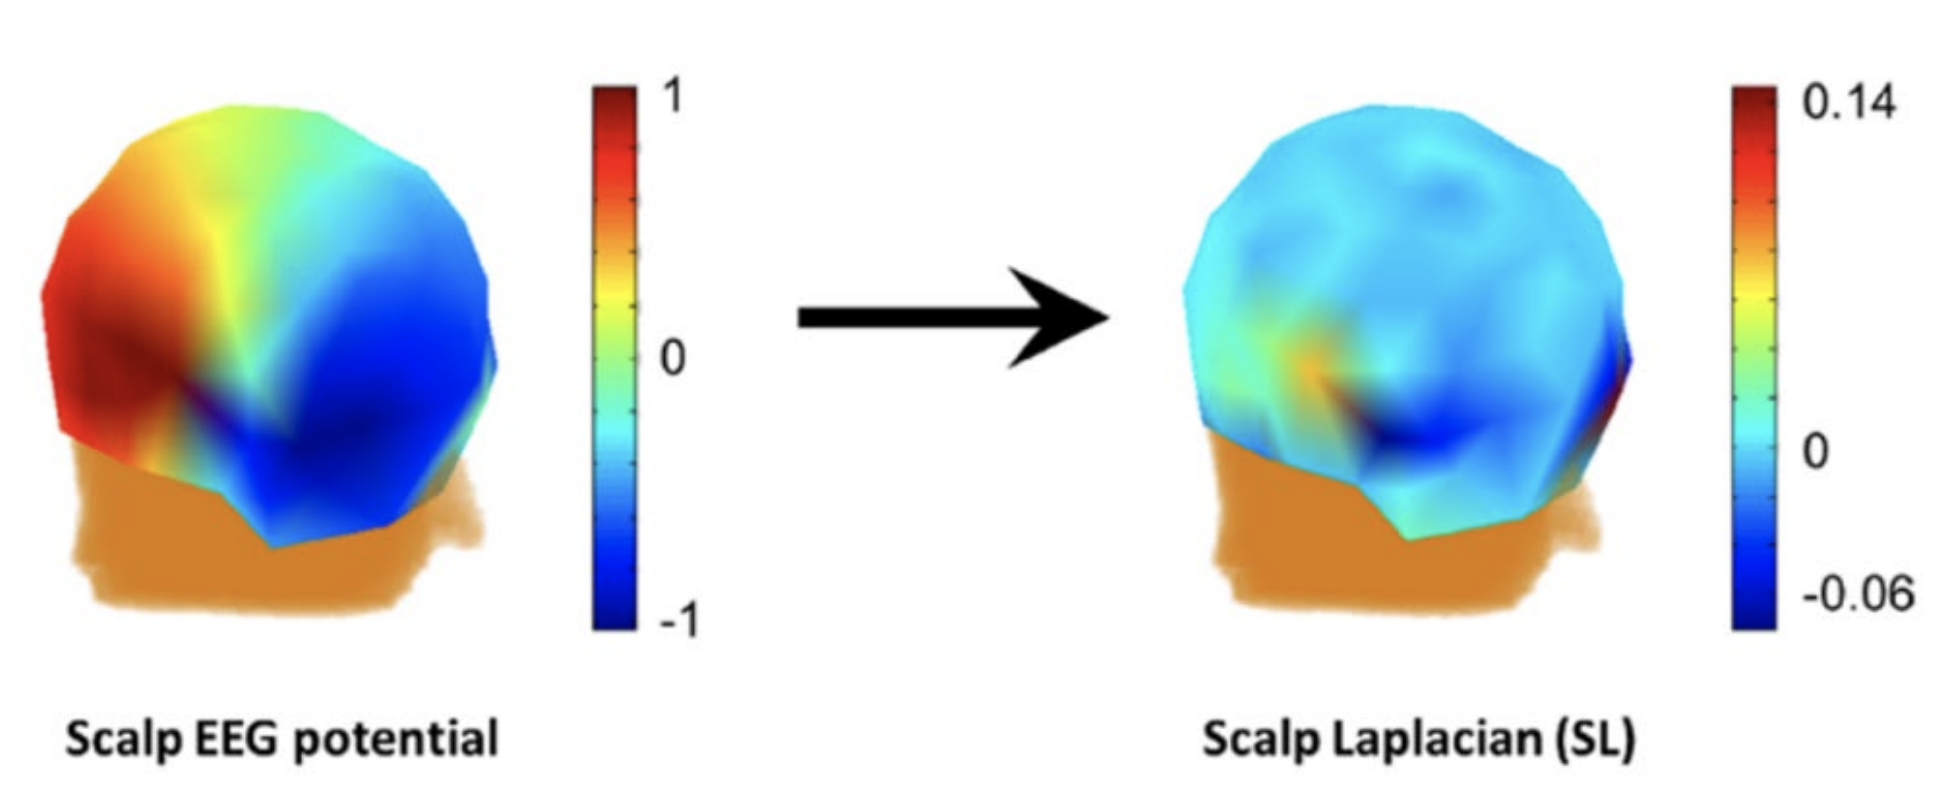
\includegraphics[width=0.6\linewidth]{images/introduction/improve_eeg_spatial_comparison.png}
    \captionsetup{width=0.9\linewidth}
    \captionsetup{justification=centering}
    \caption{Figure by \citet{improve_eeg_spatial_comparison} showing the \glspl{topomap} of the same signal at the same time but one with the use of a scalp laplacian.}
    \label{fig:improve_eeg_spatial_comparison}
\end{figure}


However, this issue is most apparent in non-invasive \glspl{bci} where electrodes are placed on the skull.
Flexible electrodes placed inside the skull to form an invasive \gls{bci}-system allow for a far larger amount of electrodes to be installed with far less obstruction from other structures.
Such an invasive system can also have far higher placement precision and requires less active-electrode amplification as the electrode is closer to the source.
This improves signal quality, spatial resolution and allows to obtain measurements from more regions of the brain that were previously blocked or too far away from the skull to be accurately measured.
State-of-the art in invasive \gls{bci} include the previous mentioned work by \citet{neuralink_whitepaper}.
Whilst theoretically such invasive systems are superior to non-invasive alternatives, they require operations to be applied and are far more expensive.
The robots build by \citet{neuralink_whitepaper} aim to automate this placement procedure making it more affordable, quicker and less dangerous.
However, the ease of use appeal and far cheaper price for non-invasive alternatives still outweigh the benefits offered by invasive methods for almost all but highly medical applications.
It has also been shown that the theoretical more precise temporal and spatial resolution doesn't linearly correlate with improved \gls{bci} accuracy/control, rather it seems to plateau relatively quickly with current state-of-the-art signal processing and classification techniques \citep{dropping_curve_eeg_lectrodes, more_electrodes_not_better}.
Some critics point to the dropping curve found by \citet{dropping_curve_eeg_lectrodes} to conclude that the increased electrodes amount and reachable neurons achieved by \citet{neuralink_whitepaper} don't have a direct impact on the usability of \glspl{bci} in real-world applications.
Nevertheless, future improvements in signal processing and classification techniques could prove invasive methods to be far superior for \gls{bci} applications and the mechanical achievements so far are not to be underestimated.

% - - - - - - - - - -

\subsection{More powerful, affordable and portable equipment}
\label{subsec:bci_gaining_popularity_better_processing}

The improvements in \gls{eeg} measuring equipment have likely been influential in the gaining popularity of \gls{bci} systems.
However, state-of-the-art \gls{bci} equipment with the highest possible resolution and accuracy remains expensive and bulky.
Complementary, as chapter \ref{ch:processing_signals} will discuss in greater detail,  working with \gls{eeg} can require some computationally heavy computations to achieve desirable classification results.
Luckily, together with the improvements in state-of-the-art equipment, there is also an emerging supply of less accurate but far more affordable and portable \gls{eeg} measuring equipment.
Due to Moore's law, \glspl{cpu} and other computational hardware have seen massive improvements in computational power as well.
This has made algorithms previously requiring expensive specialized computational hardware possible on the average personal computer.
These factors have made \gls{bci} applications, which were previously limited to lab environments with a high financial cost, accessible to a far broader public.

Early attempts at making the technology more portable and affordable include those by \citet{early_bci_drowsiness} and \citet{early_bci_multimedia}.
In essence, these applications rely on separating the \gls{eeg} measuring and data processing in two standalone systems connected over Bluetooth.
This allows for a lightweight measuring device to be placed on the user's head, with a heavier and bulkier computational unit to process the signals which ideally is still pocket-able.
The latter was not a trivial task and introduced the need for custom hardware at the time.
\citet{early_bci_drowsiness} used a custom-made \gls{dsp} for the task whilst \citet{early_bci_multimedia} opted for a more general \gls{fpga} based \gls{dsp}.
Whilst these were great demonstrations of how the technology could be used outside the lab, the actual usage for a bci detecting driver's drowsiness \citep{early_bci_drowsiness} and allowing multimedia control \citep{early_bci_multimedia} was rather limited.
The idea of custom-made and possibly proprietary processing hardware which focuses on a single task is also very limiting, although it does have commercial benefits.

What did stick, was the idea of splitting the hardware into two standalone parts, a wireless \gls{eeg} measuring device and a processing unit.
It made it possible for smaller research teams or even individuals to take part in this highly interdisciplinary field.
As an example, it enables computer scientists to purchase off-the-shelve affordable \gls{eeg} measuring hardware and communicate with it through provided libraries for their favourite programming language.
In most cases, the personal computer they already own is powerful enough for the experiments, especially for offline systems.
Section \ref{subsec:biomedical_signals_measuring_equipment} discusses some of the \gls{eeg} measuring equipment available on the market.
It is noted that \gls{eeg} measuring hardware is not strictly needed for a computer scientist as researchers such as \citet{eeg_data} have made excellent free to use \gls{eeg} datasets available.

With the introduction of the iPhone in 2007, it didn't take long for researchers to explore the idea of using a mobile phone as a processing unit for a \glspl{bci}.
\citet{early_bci_phone} were one of the first to explore this idea, with a \gls{ssvep}-based \gls{bci}.
Session \ref{sec:biomedical_signals_type_of_signals} will go into further detail on these type of signals.
In essence, such a system relies on \gls{erp}, a category of brain signals that are often easy to detect but require a specific stimulation.
This type of system can be used for a wide variety of applications.
Imagine an audio-guided tour in a museum where visitors only need to stare at a screen next to an item of interest to start hearing the explanation of that item.
This could be achieved with only a couple of dry electrodes placed on the skull in a headset that also provides the audio to the visitor.
This headset could then be connected over Bluetooth to the visitor's phone running an app for the museum tour.
The technology needed for such a system would lean close to that of so-called \textit{P300 spellers}, which have already been heavily studied \citep{p300_spellers_review, p300_keyboard_flashing, p300_spellers}.

Whilst the advantages of using the computational power of devices a customer already owns are clear, it also imposes some disadvantages.
For one, the varying type of computational devices is bound to give varying performance results and compatibility issues.
Adding to this is the added complexity for the customer of setting up the system to work with its devices himself.
From a commercial perspective, it would be easier if the system was all-inclusive and possibly patentable. 
Recent trends in computing hardware where manufacturers are shifting away from general all-purpose \glspl{cpu} and developing their custom \gls{cpu} architectures have shown that custom chips can outperform their general counterparts.
Apple's mac M series processors announced in 2020 are one such recent example.
These M series processors have a neural engine that is stated to accelerate the time needed for \gls{ml} tasks.
\glspl{gpu} used for autonomous driving systems also differ from general-purpose \glspl{gpu}.
Because of this, the author of this paper believes custom made chips could create a future where the headset has a directly integrated processing unit again.
Whilst this would make for a more attractive package for the customer and give commercial advantages to the manufacturer, it would be disadvantageous for research purposes.
The manufacturer could limit the possibilities of using the \gls{bci} for different purposes, patent promising hardware and more.
Another possible route the author of this paper sees is the use of cloud computing and fast 5G connections to also create a more simple user experience that doesn't require Bluetooth tethering to a close-by processing unit.
This approach would still leave a separation between measuring hardware and processing hardware making changes to any of the two independently easier.

To summarize, the system by \citet{early_bci_phone} was one of the earliest examples of a true portable \gls{bci}-system that was affordable and relied on a smartphone as a processing unit.
It showed how working with \glspl{bci} can be done using cheap and general-purpose hardware.
The research was published at a turning point for \glspl{bci} where publication numbers on \gls{bci}-related papers started rising.
This hints that the increased affordability and portability combined with more computational power played an important factor in the rise of interest in \gls{bci}. 
The rise of \gls{bci}-related papers is illustrated in figure \ref{fig:bci_publications}.

% Todo; change figure to include BCI work, P300 bci work and MI BCI work and ...
\begin{figure}[ht]
    \centering
    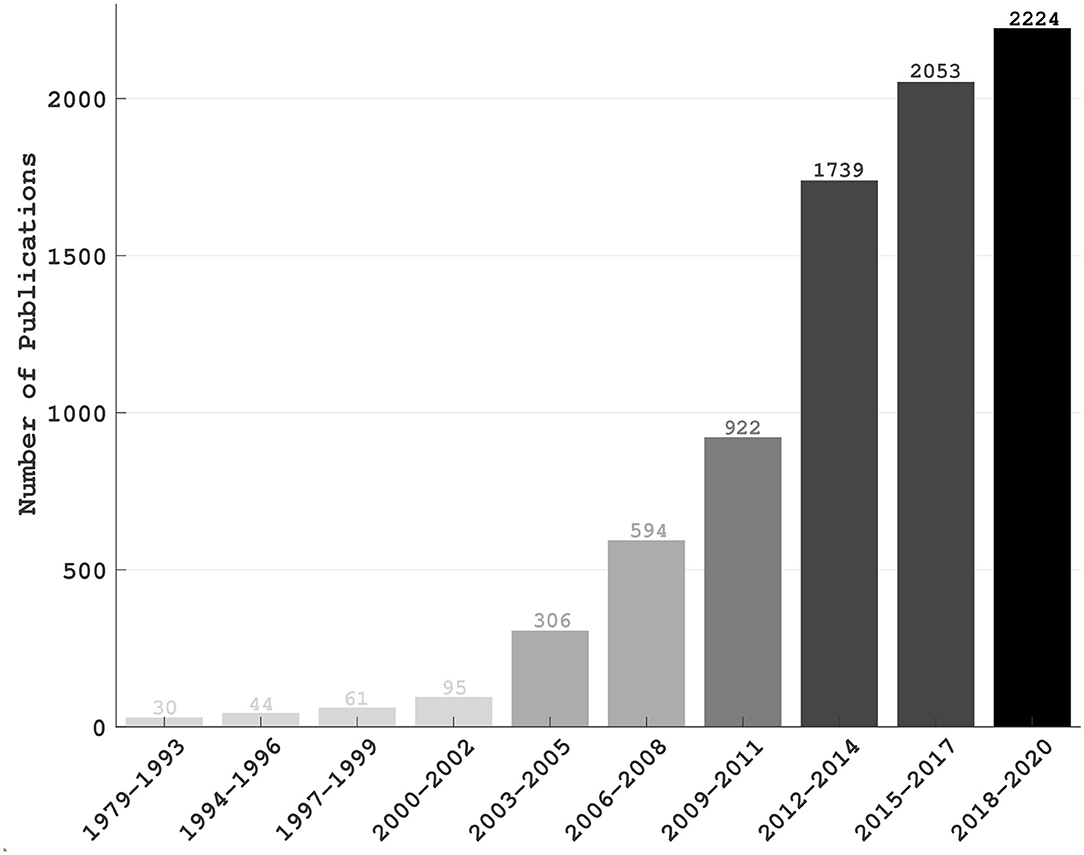
\includegraphics[width=0.6\linewidth]{images/introduction/papers_on_bci.jpg}
    \captionsetup{width=0.9\linewidth}
    \captionsetup{justification=centering}
    \caption{Number of \gls{bci}-related papers over time. Figure by \citet{bci_progress_overview} based n found papers through PubMed using the keyword: "brain computer interface".}
    \label{fig:bci_publications}
\end{figure}


% - - - - - - - - - -

\subsection{Specialized machine learning techniques}
\label{subsec:bci_gaining_popularity_improved_ml}
% TODO -- very drafty
% also EU proposal on explainable en interpretable ai 
% https://www.frontiersin.org/research-topics/13609/deep-learning-in-brain-computer-interface#overview

The previous sections discussed how better, more affordable and portable hardware has contributed to the rise of popularity for \glspl{bci}.
Another important part of the puzzle is the algorithms that convert data from these devices to useful actions.
Most of these algorithms are data-driven classifiers and rely on \gls{ml} techniques and some even incorporate \gls{dl} techniques.
These techniques and many other buzzwords under the \gls{ai} umbrella have been in the news almost daily as of late.
Because of this, these techniques often appear newer than they are.
In reality, most of these techniques evolved from decades-old ideologies.
However, a spike in data availability and the discussed exponentially improved computational power enabled these techniques to perform far better and allowed them to be used in more applications.
Combining existing techniques and relatively small tweaks to existing algorithms also gave rise to rather significant improvements.
For instance, \citet{rl_activation_function_compare} discussed how changing the activation function in \gls{rl} from CReLU to ReLU6 offered a 35\% performance increase while keeping other settings fixed for certain experiments.
This further illustrates that whilst the basic principles of such techniques are relatively old, new insights and data can make them even more powerful and applicable to more problems.

\Gls{dl} is something that has only truly become viable in a broad range of applications in the last couple of years.
Mostly due to the introduction of better libraries and faster training times due to improved hardware combined with more available data.
\Gls{dl} is not one specific technique but rather an umbrella term for techniques such as \gls{cnn}, \gls{rnn} and \gls{gan}.
Especially \gls{nn} have proven to be highly useful in many tasks including \gls{bci} applications.
Section \ref{sec:processing_signals_interpreting_ml} will go into greater detail how \gls{ml} techniques are used in typical \gls{bci} applications.

Many great \gls{ml} and \gls{dl} libraries and frameworks exist, perhaps the most famous python \gls{ml} library is scikit-learn by \citet{sklearn}.
MNE by \citet{mne} is a well-known library used for exploring, visualizing and analyzing \gls{eeg} data.
Even many \gls{eeg} classification specific \gls{ml} and \gls{dl} libraries exist \citep{eeg_model_eegnet, eeg_model_esi, eeg_model_fbcsp, eeg_model_hbm, eeg_model_ssvep}.
Publicly available datasets for \gls{eeg} data also exist, the experiments in this paper will use one by \citet{eeg_data}.
Combining these available resources makes it easier than ever to have satisfactory \gls{eeg} classification accuracy in a very reasonable amount of code and time.
These available resources are a massive bonus for the \gls{bci} field when used correctly.
The latter is easier said then done, as section \ref{sec:processing_signals_interpreting_ml} will address further when talking about \gls{ml} in \gls{bci} applications and the issues it has.

% ---------------------------------------------- 

\section{BCIs for people with disabilities and diseases}
\label{sec:bci_helping_disabled}

Previous sections addressed some of the recent commercial applications from \glspl{bci}.
Whilst these are great examples of how the technology can be used by the general population, the medical applications of \glspl{bci} remain very important to the field, if not of most importance.
\gls{eeg} signals originate from the medical field and many of the successes in the field are related to helping people with certain diseases and/or disabilities.
This section will highlight some of the major areas where \glspl{bci} can improve the quality of life for these people.

% - - - - - - - - - -

\subsection{Preventing, monitoring and controlling diseases with BCIs}
\label{subsec:bci_helping_disabled_diseases}

\Gls{eeg} trials are often used to diagnose brain disorders.
Especially seizure-related disorders such as epilepsy are often diagnosed through \gls{eeg} readouts.
But also other neurological disorders such as the locked-in syndrome rely on \gls{eeg} amongst others to be correctly identified.
Even the psychological field uses \gls{eeg} as a physiological measuring tool to aid in the diagnosis and treatment of patients, although psychiatrists should be aware of the limitations \gls{eeg} has for them \citep{eeg_for_psychiatric}.

As \gls{eeg} is used for a wide variety of diagnoses and as input data for most \glspl{bci}, much research has gone into how \glspl{bci} can be used as an aid for medical diseases.
\Citet{bci_applications} gives an overview of the most common use cases for \glspl{bci}.
In general, \glspl{bci} is used for three different reasons in medical applications: prevention, detection/diagnosis and rehabilitation/restoration.

One popular example of prevention relates to traffic accidents.
According to \citet{traffic_deaths}, traffic accidents were the number 1 cause of death for children and young adults.
Whilst many types of equipment are already in place to prevent traffic accidents from occurring, such as speed cameras and breathalyzers, it has been studied how \glspl{bci} can be used as a prevention measure as well.
The earlier discussed research by \citet{early_bci_drowsiness} that was one of the first attempts at a truly portable \gls{bci}, measured driver's drowsiness levels.
Such information can be used to alert or even enforce drivers to take a break from driving when drowsiness levels are too high.
Other research includes that by \citet{eeg_dangerous_situation_car} who has discovered that emergency situations can be classified faster from \gls{eeg} data than the user's response.
This was done through a driving simulation and was found to have an accuracy of about 70\%.
\Citet{eeg_motion_sickness} developed a system that could estimate motion sickness levels, which in turn could again be used as an alert for drivers to take a break from driving.
These three examples show how \glspl{bci} can be used in a variety of ways for the prevention of traffic deaths.
Many more applications exist for the prevention of this phenomenon and others using \glspl{bci}.

\Gls{cade} and \gls{cad} using medical imagery are widely used for diagnosis and treatment monitoring in oncology and other fields.
Comparable systems exist using \gls{eeg} data amongst others for diagnosis aids.
Whilst these do acquire and process brain signals to output a classification, the classification itself is not directly used nor is the output directly connected to other systems.
This makes calling diagnostic systems using \gls{eeg} data a stretch of the definition in some regards.
Nonetheless, the previously given example of the commercial Muse headset for sleep tracking is one example of a detection and diagnostic system that can be classified as a \gls{bci}.
It detects irregular sleep patterns, allows for diagnosing certain sleep disorders and can interact with the user to prevent or suppress the found phenomena in the future.
\Citet{eeg_sleep_apnea} have developed a similar system to detect sleep apnea from \gls{eeg}, but don't call their system a \gls{bci}.
\Citet{bci_sleep_apnea} also developed a system to detect sleep apnea but they do call it a \gls{bci}.
This shows that the definition of a \gls{bci} is not strict.
However, all of these systems make use of similar methodologies compared to more clear \gls{bci} systems.


% reset emg gls
\glsreset{emg}

Restoration of lost mobility and environmental control is where \glspl{bci} shine.
As most prostheses rely on \gls{emg}, a muscle-based \gls{biosignal}, for controlling them, they do not apply to patients who don't have muscle control anymore.
Luckily, \gls{bci} are often used as novel interaction methods using brain signals, which enables such patients to regain previous levels of mobility and control.
Section \ref{subsec:bci_helping_disabled_extending_medical_system}, \ref{subsec:bci_helping_disabled_prostheses} and \ref{subsec:bci_helping_disabled_novel_interaction} give some more insight on how \glspl{bci} are used regain lost mobility and environmental control.
As \citet{bci_rehabilitation} discuss, \glspl{bci} can also be used to guide patients in rehabilitation through brain plasticity.
Brain plasticity, or neuroplasticity, is the brain's ability to adapt itself based on experience.
\Glspl{bci} could show patients which regions of the brain are used and which types of brain signals are present.
This information could then be relayed to the patient through various means so that it induces neuroplasticity.
Such systems are still in development and require sophisticated neurological expertise that falls outside the scope of this master thesis.
The overview provided by \citet{bci_rehabilitation} provides a great starting point for further literature on this manner.
In a similar manner, pedaling \glsfirst{mi} tasks have been studied recently as they seem to have a great potential for lower-limb recovery.
The works by \citet{pedal_mi_rehabilitation1} and \citet{pedal_mi_rehabilitation2} discuss such systems in greater detail and are also an example of how \glspl{bci} can be used for rehabilitation.

It is noted that many more \gls{bci} applications exist for preventing, monitoring and controlling diseases than those discussed.
The work by \citet{parkinson_stroke_reduction} is another great example of how \gls{bci} can be used for rehabilitation.
The work by \citet{bci_in_medicine} also highlights some related \gls{bci} work in medicine.

% - - - - - - - - - -

\subsection{Using BCIs to extend existing medical systems}
\label{subsec:bci_helping_disabled_extending_medical_system}

\Glspl{bci} can be used in a wide variety of applications.
Even in non-trivial domains, they can find their usages as a standalone system or as an extension to existing systems.
To demonstrates the latter, this section discusses how \glspl{bci} can be used as an extension to classical hearing aids for an improved user experience.
A more trivial extension to existing robotic prostheses and exoskeletons is also addressed.


According to \citet{hearing_aids_noise_reduction} over 450 million people suffer from disabling hearing loss.
Most solutions to hearing loss rely on a microphone to capture environment audio which is then amplified and played through a speaker that is placed in or near the ear.
This microphone can be integrated inside the speakers and thus form a stereo setup located at the ears of the patient.
This is not always ideal when there is a lot of ambient noise.
Sometimes using an external directional microphone placed close to the audio source of interest can form a solution.
This can be a microphone placed on the desk of a professor teaching in a filled room or the speakers connected directly to an audio source such as a television.
However, this solution is not applicable in all situations.
Thus, most hearing aids include some noise suppression on the microphones directly to filter out ambient noise and amplify noise coming from human speech.
\Citet{hearing_aids_noise_reduction_mandarin} evaluated such noise suppression for Mandarin-speaking users and found the results to be good but not ideal.
\Citet{bci_hearing_aid_direction} have shown that a \gls{bci} can be used to determine which speaker a user is listening to by analysing directional queues.
This information is useful, as it can optimize the microphones to pick up speech from that area and algorithms could optimize for the sounds the user is focusing on.
It is noted \citet{bci_hearing_aid_direction} discuss how a long waiting time to determine the area of interest challenges the practical usability of their system as of now.
Nonetheless, it shows one of many non-trivial ways a \gls{bci} could be used as an extension of existing systems to improve them.

% reset emg gls
\glsreset{emg}

Perhaps the most studied and promising extension \glspl{bci} can fulfil in existing medical systems lies in the interaction with robotic prostheses or exoskeletons.
Most of the current robotic prostheses and exoskeletons rely on muscular activity in the body.
This muscular activity can then be measured by \gls{emg}, the data of which can be used to control the robotic prosthetic.
For example, patients who have lost (part of) their arms but have functioning muscular activity in the remaining body part, can use this remaining muscular activity to control robotic prostheses.
\Citet{emg_prosthetics} discuss the design and development of such a system based on \gls{emg}.
Some of the processing techniques are similar to those of \gls{eeg} driven algorithms.
Alternatively, when the limb is still intact but the control over (part of) the limb is lost or extra support is needed, an exoskeleton may be used.
Just like robotic prostheses, most exoskeletons rely on \gls{emg}.
A thesis by the German \citet{emg_exoskeleton} highlights the fundamentals of \gls{emg} based exoskeletons.

As was already touched upon in section \ref{subsec:bci_helping_disabled_diseases}, \gls{emg} measurements are not applicable for all patients.
In particular, people who have neurological diseases limiting the production of the required muscular based \glspl{biosignal} fall outside the scope for these solutions.
However, due to the developments in \glspl{bci}, the viability of robotic prostheses and exoskeletons for these patients has been steadily on the rise.
\Citet{bci_prostheses} give an in-depth systematic review of upper and lower limb exoskeletons and robotic prostheses controlled by \gls{eeg}-based \gls{bci}.
\Citet{bci_prostheses} address the high risk associated with failed instructions for robotic prostheses and exoskeletons.
Indeed, compared to a misclassification with P300 spellers, the risks that can follow from misinterpreted instructions of exoskeletons and robotic prostheses are of such a degree that even high accuracy systems might not be good enough.
\Citet{bci_prostheses} also highlight that whilst multi-label classification of \gls{eeg} is possible with considerable accuracy in an offline lab setting, the number of detectable classes is limited in a real-time and real-life environment.
Because of this, \gls{eeg}-based systems in these applications still have some challenges to overcome to match the precision and reliability of \gls{emg} counterparts.
Whilst improvements regarding these aspects have been made since the work of \citet{bci_prostheses} was published, the main challenges remain to this day, especially when using affordable systems.
Because of this, widespread adoption of \gls{eeg}-based exoskeletons and robotic prostheses is still very limited.

% - - - - - - - - - -

\subsection{Novel interaction methods using brain-signals}
\label{subsec:bci_helping_disabled_novel_interaction}

The previous section highlighted how \glspl{bci} can be used to extend existing medical systems.
When working with exoskeletons and robotic prostheses, the \gls{bci} systems provide a novel interaction method for these devices that normally rely on \gls{emg} or other sources for input.
Many of the successful \gls{bci} applications consist of providing novel interaction methods with existing systems.
It could be argued that almost all of the literature proposed \gls{bci} applications boil down to making a novel interaction method of some sort.
Opposed to the discussed \gls{eeg}-based exoskeletons and robotic prostheses, whose risk currently leads to limited real-life applications, less risk imposing \gls{bci} applications do find their use as novel interaction methods in real-life already.

The P300 spellers discussed earlier are examples of novel interaction methods that aim to replace keyboards, especially for those who don't have the required capabilities to operate them \citep{p300_spellers, p300_spellers_review}.
Whilst wrong classifications in a speller application could result in unpleasant situations, it is clear that the risk involved is far smaller than exoskeletons for example.
As the name suggests,  P300 spellers make use of \textit{P300 signals} which are a type of \glsfirst{erp}.
As is further discussed in section \ref{subsec:biomedical_signals_type_of_signals_erp}, a P300 signal is a positive bio-electrical wave measurable with \gls{eeg} around 300ms after a stimulus occurred.
The stimulus used is often a flashing pattern on a monitor, of which there are multiple shown in a matrix form.
The users have to focus on the element of the matrix that they want to select and appropriate algorithms can extract this selection from \gls{eeg} data.
\Citet{p300_speller_real_life} performed a usability study on 20 \gls{als} patients in a real-life like environment.
According to \citet{p300_speller_real_life}, most participants achieved over 70\% accuracy, which is in line with the findings of \citet{p300_spellers_review} and \citet{p300_speller_real_life2} in similar studies amongst other types of patients.
More interestingly, even though the accuracy wasn't extremely high, all participants of the experiment by \citet{p300_speller_real_life} succeeded in the given tasks.
This is in part due to our ability as a human to understand typo's in words and sentences relatively easily.
Another important factor is that most of these systems make use of auto-correct software to help combat faulty classifications.
Besides auto-correct software, state-of-the-art text prediction is also a crucial part of these systems as it can almost double the efficiency of P300 spellers.
\citet{p300_speller_real_life} has found that the use of word predictors raised the mean number of correct symbols per minute from 3.6 to just over 5.
Whilst 5 symbols per minute is still a lot slower compared to regular keyboard input, it enables useful communication for those who can't communicate through regular means.
As \citet{p300_speller_real_life2} have shown, P300 spellers can be used by \gls{als} patients with satisfactory results in a pleasant manner for the user.
\Citet{p300_speller_real_life2} have shown equal results for \gls{dmd} patients.
In general, P300 spellers are often used as they have a low learning curve that can quickly enable a patient to regain some communication skills.
The reason these systems have a low learning curve and can be quickly deployed is due to their simple user interface and a combination of a system that generalizes well and that has been studied thoroughly for the use of \gls{tl}.
Early examples of using \gls{tl} for P300 related \glspl{bci} include those by \citet{p300_speller_tl}.
It is noted that eye-tracking is a viable alternative for P300 spellers in most cases and research has been put into combining the two, such as the work by \citet{p300_eye_tracking_speller}.

The focus on user experience by \citet{p300_speller_real_life2} is an important factor of a real-life case study.
User experience is often overlooked by initial \gls{bci} system proposals, where the focus is often on numerical measures such as accuracy, speed and \gls{fn} or \gls{fp} rates.
However, good working \glspl{bci} can cause psychological burden and other side-effects on the patients using them which an initial \gls{poc} might not reveal.
This gives rise to some ethical challenges, some of which are discussed in section \ref{sec:bci_ethical}.
As time passes, the user might move to a more capable and sophisticated system that has a steeper learning curve, higher cost and is more demanding for the user.

As P300 signals are relatively easy to detect through \gls{eeg}, it is one of the most studied signals from \glspl{erp}.
Many other \gls{bci} applications are based on P300 signals then just spellers.
One such example is the \textit{Facebrain} application by \citet{facebrain}.
Facebrain provides an \gls{eeg}-based novel interaction method with the social media platform Facebook.
In essence, it's a regular P300 speller with the first screen(s) representing possible actions to take on the platform.
When text input is required, a regular P300 speller user interface is presented.
This allows a user to operate almost all of Facebook's functionalities with only a P300-based \gls{bci}.
The application by \citet{facebrain} is one of many that shows the same strategy and classification algorithms as P300 spellers can be used for a wide variety of applications by changing the meaning and functionalities of the shown matrix elements.
The matrix elements could even be overlapped on top of an image to have intuitive motion control, a methodology used by \citet{p300_drone} for their P300 controlled quad-copter.

\glspl{erp} and the measurable signals they produce, such as the P300 signal, are only one of many sources for detectable brain signals.
In general, \gls{erp} related signals are easier to detect reliably, as the stimulus can be controlled, giving a hint when and where to look for signals and what to look for.
However, P300 and \glspl{erp} in general also have their issues and limitations.
The \gls{bci} handbook by \citet[Chapter~26]{bci_handbook} discusses the crowding effect, adjacency problem, repetition blindness and user discomfort amongst other issues \glspl{erp} have.
Most problems arise from the often limited space for sending stimuli without overlap and the changing behaviour of both the brain and participant's experience after a prolonged session where many stimuli have been applied.

An alternative to \glspl{erp} is using a mental phenomenon called \gls{mi} as source of signals for a \gls{bci} system.
\Gls{mi} is the process in which a person generates brain activity in the motor cortex merely by imagining motor movements.
Section \ref{subsec:biomedical_signals_type_of_signals_motor_imagery} explains in further detail how \gls{mi} is not dependent on an external stimuli nor actual motor movements.
This makes \gls{mi}-based \glspl{bci} extra appealing as they don't require external stimuli and are applicable for people with motor disabilities.
\Citet{first_mi} were the first to experiment with the idea of using \gls{mi} in an \gls{eeg} classification task.
Since then, many \gls{mi}-based \glspl{bci} have been proposed.
\Citet{bci_mi_robot_arm} proposed a \gls{mi}-based \gls{bci} to control a robot arm system.
Their research is interesting in two ways.
First, they use only three distinct \gls{mi} classifications: imagined right-hand movement, imagined left-hand movement and imagined foot movement.
These three controls enable the user to select eight different possible actions through a menu where two options are always shown that can be controlled using either an imagined left-hand movement or an imagined right-hand movement.
Scrolling through the menu to show two other possible actions is possible through the imagined foot movement.
This shows that with the right system design few controls can still allow for many actions to be taken.
Secondly, they found that experienced users have better overall classification performance which indicates that \gls{mi} is something that can be trained.

A more recent and more complex \gls{mi}-based \gls{bci} system is the vehicle control system by \citet{bci_mi_four_wheel_drive} which recognizes four possible actions: left, right, throttle and brake.
There are three very interesting aspects in the work by \citet{bci_mi_four_wheel_drive}.
First, they use two distinct classifiers for the \gls{eeg} data.
One makes a distinction between left and right through a typical \gls{mi}-based \gls{bpnn} whilst the other classifies throttle and brake behaviour using the subject’s threshold value of the average band power.
Secondly, an additional system is in place to reduce the risk of wrong classifications in the system.
This additional system is a type of collision detection and avoidance system that uses four ultrasonic wave radars and a camera.
The rationale behind this additional system is that the car would operate more like a semi-autonomous system that is responsible for a safe ride whilst the input of the \gls{bci} system is used to steer this semi-autonomous car in the right direction.
This additional system is required as the accuracy of around 84\% for the throttle and brake classification and 89\% for the left and right classification is not enough for a reliable system.
Finally, they use an interesting data collection method to train the classifiers on a user-per-user basis.
They configured a driving simulator where the user has the freedom to perform any action they want through a classical steering wheel and pedal setup.
The user should synchronously think about the action they want to perform to generate \gls{mi} data and they have to perform the effective action, as to be able to label the data.
Whilst this is an interesting approach, it is limited in the fact that it requires the user to be able to operate a steering wheel and pedals at the same time, which is not the case for classical target users of these systems.

Far more types of brain signals exist for use in \glspl{bci} than those discussed in this section.
Section \ref{sec:biomedical_signals_type_of_signals} will go into further detail on the different types of brain-signals that can be used.
For a more exhaustive list of all different approaches to using \glspl{bci} as novel interaction the reader is advised to consult one of many systematic reviews, books and other materials already available \citep{bci_review_book_chapter, bci_review, bci_in_medicine, bci_history, bci_review_monkey, bci_handbook}.
From the works these materials discuss, it should become apparent that most short-term goals of \glspl{bci} still lie in improving the quality of life for people with disabilities.
However, the rise in popularity of \glspl{bci} in the gaming industry and amongst other big tech companies as discussed in section \ref{subsec:bci_gaining_popularity_big_tech} shows there is a potential future where \glspl{bci} find more real-life use-cases in other fields as well.
Many of the current research also looks into combining multiple technologies to limit risk, increase the number of classification classes, create a more pleasant training experience and more.
It is important to stress that the research field of \glspl{bci} is not as new as some of the more commercial companies and publishers would like to portray it is.
Because of this, some of the claimed breakthroughs should be taken with a grain of salt.
One such example is the use of \glspl{bci} with monkeys.
Neuralink, the earlier discussed Elon Musk company, has published a YouTube video\footnote{\url{https://www.youtube.com/watch?v=rsCul1sp4hQ}} in 2021 demonstrating a monkey playing pong using the \gls{bci} by Neuralink.
The video quickly gained millions of views, far more than most papers in the \gls{bci} field will ever reach.
As a result, this video without a backing paper or proper explanation of the process was covered as highly innovative and groundbreaking by many news outlets.
However, similar setups have already been made in the past.
For example, \citet{bci_monkey_arms} demonstrated monkeys taking control over two avatar arms simultaneously, a task that is arguably even harder to accomplish and has an appropriate peer-reviewed paper backing it.


% - - - - - - - - - -

\subsection{Using BCIs with and as prostheses}
\label{subsec:bci_helping_disabled_prostheses}


It was argued in section \ref{subsec:bci_helping_disabled_extending_medical_system} that the risk involved when working with exoskeletons and robotic prostheses is too high for current \gls{bci} systems to be reliably used.
The \gls{bci} controlled car from \citet{bci_mi_four_wheel_drive} discussed in section \ref{subsec:bci_helping_disabled_extending_medical_system} demonstrated how risk of a \gls{bci} system can be greatly reduced by using an additional system responsible for only allowing safe actions.
Similar ideas could be used for robotic prostheses to reduce the risk involved.
\Citet{bci_mi_robotic_arm_collision_avoidance} proposed such a hybrid system to control a robotic arm not only through a \gls{mi}-based \gls{bci} but also by using obstacle avoidance algorithms to reduce the risk of harmful contact, computer vision for object detection to get a better idea on the wanted interaction and eye-tracking to gather extra information surrounding user's intention.
Hybrid systems like the one by \citet{bci_mi_robotic_arm_collision_avoidance} are very promising as they can greatly reduce the risk involved in many \gls{bci} systems, such as prostheses related applications, whilst also increasing the overall accuracy of the system.

Whilst limb prostheses such as robotic arms are one of the most common types of prostheses, they are only a fraction of all prostheses in existence.
Everything from dentures and hearing aids to artificial breasts can also be labelled as a type of prostheses.
Visual prostheses such as bionic eyes are another type of prostheses and they are being studied heavily in the \gls{bci} field.
Not only can \gls{bci} systems improve visual prostheses, many of the existing visual prostheses could be seen as a special type of \gls{bci} system as a whole.
Both the works by \citet{bci_blind_assist_review} and \citet{bci_vision_assist_review} give an overview on the progress in visual prostheses in the \gls{bci} field.
These \glspl{bci} are often invasive that can stimulate the brain and other parts of the body, as opposed to only reading brain activity.
Through the simulations or other means, the user can regain some form of vision from these \gls{bci} systems.
Second Sight is one of few companies that has commercially made visual prostheses with \gls{fda} approval.
It is discussed in the overview on \gls{bci}-related vision restoration systems by \citet{bci_vision_assist_review}.
The international trial by \citet{second_sight_trial} on the products of Second Sight shows promising results, although it is noted the study is performed by Second Sight employees and not by an independent research team.
The exact working of visual prostheses or, more specifically, Second Sight products is not of interest for this work, but the recent decisions of Second Sight company reveal one of the largest risks of invasive \glspl{bci} and \glspl{bci} in general.
Due to the discontinuation of some of the Second Sight products, hundreds of users are left without product support for a system that shaped their everyday life.
Besides this, the now non-functioning product is still present inside their body.
The issues and ethical questions this brings to the table are discussed further in section \ref{subsec:bci_ethical_e_waste}.

% ---------------------------------------------- 

\section{Small projects with large potential}
\label{sec:bci_small_projects}

As technology evolves, it has often been the case that people with certain disabilities benefit from the evolution as well.
Take the evolution of live captions as a recent example, it has found its way directly into the Android smartphone operating system.
Whilst initially implemented for users to enjoy video content in situations where they can't listen to the audio, people with hearing difficulties now have a direct way to enjoy more content too.
The push for autonomous cars will allow those that are traditionally unable to drive a car to finally enjoy the freedom a car can offer as well without being dependent on others to do so.
Object and scene recognition algorithms made for optimizing smartphone cameras can also be used as a way of describing what is on a photograph for those who have limited vision.

Whilst it is clear from the previous sections that research in \glspl{bci} has its roots in medical applications, more commercial applications are currently being explored as discussed in section \ref{subsec:bci_gaining_popularity_big_tech}.
These commercial applications have a larger potential audience, which will probably result in more sales.
In general, hardware and software that is produced and used on a larger scale cause market competition which in term often lowers prices whilst increasing quality.
This is bound to also make medical-oriented applications of \glspl{bci} more accessible and of better quality.
It would also allow for smaller creators with a limited budget to create meaningful, quality-of-life improving applications.
This has been the case with smartphone applications for a long time.
Simple applications such as a colour picker in the camera app can aid people who have colour blindness in determining whether a banana is ripe or not.
Small applications by individual developers relying on location changes can remind those with short-term memory loss if they have not forgotten essential things such as locking the door.


More and more open-source \glsfirst{dl} libraries tailored towards \gls{eeg} such as the ones by \citet{eeg_model_hbm} and \citet{eeg_model_eegnet} have been introduced.
These \gls{dl} libraries can often work on raw \gls{eeg} data directly, which allows developers who don't have much domain experience to make interesting and good performing classification pipelines or even make new discoveries in the field.
Publicly available \gls{eeg} dataset such as the one by \citet{eeg_data} makes it possible for developers to work on a pipeline without needing the monetary investment in \gls{eeg} measuring equipment.
If desired, the affordable headsets by OpenBCI and others, further compared in section \ref{subsec:biomedical_signals_measuring_equipment}, make it possible to have \gls{eeg} measuring equipment with good open-source libraries for well under 1000 euros.
These smaller projects do not only have the potential to be of big impact for very specific users, they often reveal common issues and interesting alternative approaches in the \gls{bci} field.

% - - - - - - - - - -

\subsection{Motivating examples using consumer-grade BCIs}
\label{subsec:bci_small_projects_motivating_examples}

As discussed above, good open-source libraries, datasets and even measuring hardware have made the entry to the \gls{bci} field easier than ever before.
Some of the open-source \gls{dl} libraries tailored towards \gls{eeg} classification work well on raw \gls{eeg} data, which allows for meaningful classification accuracy without the need of understanding all domain-specific properties of \gls{eeg} data required for classical preprocessing.
The question remains whether which or even if, real-life applications are possible on consumer-grade \gls{bci} systems.
In an ideal world, such applications should be fully configurable and usable by the end-user without the help of a domain expert and the system should be maintainable without exhaustive preliminary knowledge. 
Many works have demonstrated the potential of these \gls{bci} systems but the lack of widespread adoption suggests there are still hurdles to overcome for them to become a reality.
For this reason, this thesis focuses on providing a solid foundation to the \gls{bci} field, a \gls{poc} application to demonstrate how a working system can be implemented and a thorough viability discussion of these systems in their current state.

Multiple studies comparing different aspects of these cheaper consumer-grade systems to the more traditional medical-grade \gls{bci} systems have already been done, as is further discussed in section \ref{sec:biomedical_signals_measuring}.
In general, cheaper systems work with a lower electrode count and those electrodes also have a lower signal quality.
Whilst this means the hardware is of lower quality, cheaper consumer-grade systems can reach usable levels of accuracy as shown by \citet{openbci_vs_medical} and \citet{openbci_eeg_sensor_evaluation} for the Texas Instrument ADS1299 chip, commonly found in consumer-grade hardware such as the offerings from OpenBCI.
Similarly, studies have been done on different types of electrodes as already touched upon in section \ref{subsec:bci_gaining_popularity_better_measuring} and further discussed in section \ref{subsec:biomedical_signals_measuring_equipment}.
These electrode comparison studies have shown that the gap between easy-to-use and affordable dry electrodes and the more superior but harder to use and often more expensive wet electrodes is shrinking \citep{wet_vs_dry, dry_electrode_status, wet_dry_comparison_experiment}.
However, these findings often follow from very controlled experiments in lab-like environments.
This is to be expected, as most comparisons aim to eliminate as many random factors as possible.
However, this means that these experiments don't give great insight into the real-life usability and applicability of these cheaper \gls{bci} systems.
This section will focus on some work that demonstrates which real-life applications are possible on consumer-grade \gls{bci} hardware and how they are possible.
These works were motivational examples for this master thesis.
They give a more thorough vision of what types of applications could be possible with consumer-grade systems in their current form, often highlighting the issues that are still present with them.
Most of these works are centred around OpenBCI hardware, the manufacturer of some of the more successful low-cost \gls{biosignal} measuring devices as further discussed in section \ref{sec:biomedical_signals_measuring}.

% | | | | | | | | | | | | |

\subsubsection{Step-by-step implementation of a binary MI classification model by Peterson et al}
\label{subsubsec:bci_small_projects_motivating_examples_binary}

\Citet{cheap_bci_feasibility} aimed to show the feasibility of a complete low-cost consumer-grade \gls{bci} system.
\Citet{cheap_bci_feasibility} did this by discussing the steps required to make an offline binary \gls{mi} classification system using common low-cost consumer-grade hardware.
The classification distinguished the \gls{mi} task of a grasping movement with the participants' dominant hand and a rest condition.
They compare three different approaches in growing complexity: \gls{csp}, \gls{pfbcsp} and \gls{ptfbcsp}.
The work by \citet{cheap_bci_feasibility} has five interesting aspects worth highlighting here.

First, whilst they did use the OpenBCI Cyton and Daisy board they did not use the 3D printable Ultracortex Mark IV headset from OpenBCI.
They argued that this is due to the Ultracortex Mark IV headset becoming uncomfortable quickly due to the use of dry electrodes combined with limited adjustability.
This complaint on user comfort for the Ultracortex Mark IV headset is recurring with other authors including the one from this master thesis.
Because of this, they opted for wet EEG electrodes attached to a very flexible and far more comfortable Electro-Cap.
\Citet{cheap_bci_feasibility}  opting for wet electrodes is slightly odd, considering the user experience of having to apply a conductive gel before each use is not great and therefore not favourable for general real-life \gls{bci} applications.

Secondly, for the data gathering of their system \citet{cheap_bci_feasibility} used a \textit{common office room}, rather than a lab-like environment.
Except for a 3D printed holder for the OpenBCI board, there was no specialized shielding in place to protect the electrodes or OpenBCI boards from unwanted interference.
They argue this makes the data more realistic, and whilst true, it is important to note there is still far less stochasticity than there would be in real life.
The office room and hardware were identical for each of the participants in the data collection stage.
The room was free of external stimulus as it was separated from the experiment organisers and the participant was \textit{left alone} for the entire trial.
All participants were right-handed and thus the dominant hand used for the \gls{mi} task was always the right hand.
Adding to all of this, the dominant hand of the participant was placed inside a box to not allow them to see their hand.
It could be argued these factors still make the data more lab-like than home-like.
Still, \citet{cheap_bci_feasibility} found that the non-shielded regular office caused significant noise.
In one trial the electromagnetic noise amplitude (50 Hz or 60 Hz depending on location) was four times higher than the meaningful EEG data.
Other types of noise were also present, proving their environment was indeed far less ideal than a lab environment, which indeed makes it more realistic.

Third, during the data collection, a \gls{emg} system was also in place.
This \gls{emg} system was used to filter out samples of the collected \gls{mi} data where the movement was also physically performed, meaning it wasn't true \gls{mi} data.
Whilst this forms an interesting approach to data filtering when collecting training samples, the extra needed hardware that is only used during training is probably a tough sell in a commercial application.
However, it does automate the data filtering process used, which is more realistic for widespread use than the expert-based data filtering in most literature. 

Fourth, they used the KVIQ-10 questionnaire by \citet{kviq} to determine how \textit{good} a participant would be in \gls{mi}, a task that is proven to be harder for some individuals.
Interestingly, \citet{cheap_bci_feasibility} found no statistically significant correlation between the KVIQ-10 score of participants and the found classification accuracy.
Thus, whilst they did find significant inter-participant differences in accuracy, determining beforehand if a participant will have pleasant accuracy results beforehand through the KVIQ-10 questionnaire by \citet{kviq} wasn't reliable for \citet{cheap_bci_feasibility}.
This is an issue, as knowing this information beforehand can give a potential buyer a better indication if the system would be fit for them or not.

Finally, even though the data acquisition happened under guidance in the work of \citet{cheap_bci_feasibility}, there were still issues with the recordings.
Out of the 12 participants, there were multiple moments where connection loss with the OpenBCI main board occurred, one participant where a mechanical defect rendered the data useless and one where there were \gls{emg} detected movements of the hand for more than half of the \gls{mi} tasks rendering the trial of that patient useless as well.
Whilst the latter is an issue independent of the hardware used, the other two are probably bigger issues on the cheaper hardware than the more reliable medical-grade hardware.
Part of the reason medical-grade hardware is about 5 to 10 times as expensive for a similar experiment is due to the medical-grade hardware requiring certifications, which also guarantee some form of quality and reliability. 

To conclude, the work by \Citet{cheap_bci_feasibility} discusses the creation of a complete low-cost consumer-grade \gls{bci} system.
This system consists of the OpenBCI measuring equipment where the dry electrodes on the 3D printed Ultracortex Mark IV are replaced with electrodes in a more comfortable Electro-Cap.
The effective classification of the system is a binary \glsfirst{mi} classification on whether or not the participant imagines a grasping movement of the hand or not.
\Citet{cheap_bci_feasibility} achieved an average accuracy between 70\% and 85\%, being higher as the approach used becomes more complex.
It is important to note that the evaluated models are on a patient-per-patient basis.
This means that each patient has their own uniquely trained model and that data from the same patient is used in the evaluation process.
Whilst the binary nature of the system makes it hard to find viable real-life applications, the performance reached is almost identical to those of medical-grade systems and follows from a less lab-like environment than is typically the case.
The system proposed by \Citet{cheap_bci_feasibility} is of less importance in their work, rather the steps and pitfalls highlighted are of value.



% | | | | | | | | | | | | |

\subsubsection{Multiclass classification methods for motor imagery EEG data}
\label{subsubsec:bci_small_projects_motivating_examples_mi_classification}

The above discussed paper by \citet{cheap_bci_feasibility} provides great insight on the steps required to develop an \gls{eeg}-based consumer-grade \gls{bci} which uses \gls{mi} related signals.
Since \citet{cheap_bci_feasibility} uses a binary classification model, there are only two possible outputs of the classifier, which is too limited for most applications.
However, the lack of training samples combined with noisy and often high-dimensional data of \gls{eeg} makes multi-class classification considerably harder than binary using any \gls{bci} system.
Adding to this, the consumer-grade hardware suffers even more from noise and \gls{mi} data is notorious for being noise-prone in \gls{eeg} data.
This makes the choice for a binary classifier by \Citet{cheap_bci_feasibility} understandable.
\Citet{cheap_bci_feasibility} also opted for an approach where a model is trained per user.
This is often done in the field as it makes for far higher accuracy for that specific user.
This does however mean that each new user should also undergo a training data collection procedure to have a custom-trained model as well before being able to use the system.
This is less than ideal for commercial \gls{bci} systems and can have a physiological burden in medical applications.

To combat these points, many multi-class classification pipelines have been proposed in literature that work well with \gls{mi} related \gls{eeg} data \citep{fbcnet, eeg_mi_model_mussi, eeg_mi_model_lda_csp, eeg_mi_model_deep_cnn_spatial_filters, eeg_mi_model_image_based, eeg_model_fbcsp, eeg_model_hbm, eeg_model_esi, eeg_model_eegnet}.
These pipelines generally work on both consumer-grade and medical-grade systems, although consumer-grade systems can often benefit more from specific noise-reduction steps in the pipeline.
Some of the proposed pipelines also focus on generalisation to allow a general model which has usable performance for completely new users.
Whilst such models have poorer performance overall, they can be used as an initial model to allow the user to explore the possibilities of the \gls{bci} model without having to undergo the often tedious training data collection process. 

A complete in-depth review of all of the different approaches that can be taken to classify \gls{eeg} data falls outside the scope of this research paper.
\citet{eeg_analysis_methods_epilepsy_review} compared \glsfirst{lr}, \glsfirst{ann}, \glsfirst{svm} and \glsfirst{cnn} for a binary classification task of either being epileptic \gls{eeg} data or not.
Whilst this is again a binary classification that is more tailored towards \glsfirst{cad}, the techniques used in the experiments are also often used in the multi-class classification of \gls{eeg} data for other \gls{bci} purposes.
\Citet{eeg_analysis_methods_epilepsy_review} found that \glspl{ann} performed best for their classification task.
In general, \glspl{ann} and other \gls{dl} models such as \glspl{cnn} have proven to be successful at \gls{eeg} data related tasks.

Because of this, many of the current state-of-the-art models for \gls{eeg} classification rely on \gls{dl} models.
Especially classification pipelines that include \glspl{cnn} have proven to be successful for \gls{eeg} classification.
From the previously referenced pipelines, \citet{fbcnet, eeg_mi_model_mussi, eeg_mi_model_deep_cnn_spatial_filters, eeg_model_hbm, eeg_model_esi, eeg_model_eegnet} make use of \glspl{cnn}.
Although \glspl{cnn} are only part of a good \gls{eeg} classification pipelines.
\Citet{fbcnet, eeg_model_fbcsp} used \glspl{cnn} after a Filter-Bank approached, which has satisfactory accuracy for \gls{eeg} classification and \gls{mi}-related \gls{eeg} data in specific.
Some complex pipelines that rely on \gls{cnn} can be too demanding for real-time classification, something that is needed for an online \gls{bci} system.
Pipelines such as the one by \citet{eeg_model_eegnet} have been developed to use \glspl{cnn} in such a way that real-time classification is possible.

\glsreset{csp}
Other types of pipelines incorporate techniques based on spatial patterns, with \glspl{csp} being a very popular method used for \gls{eeg} data.
The pipelines by \citet{eeg_mi_model_lda_csp, eeg_mi_model_deep_cnn_spatial_filters} use such spatial pattern techniques, as well as the previously discussed work by \citet{cheap_bci_feasibility}.
a \gls{csp} approach is often combined with a \gls{cnn} for classification but can also be combined with more classical \gls{ml} techniques such as a \gls{svm} model or a \gls{lda} \citep{eeg_mi_model_lda_csp}.

As discussed, many approaches to \gls{eeg} data classification exist and not all of them can be listed here.
Some more noteworthy pipelines include the one by \citet{eeg_mi_model_image_based}.
Their approach is interesting in the fact that it visualizes \gls{eeg} data so that an image processing method can be used for classification.
Whilst this yields okay results, it doesn't improve upon the state-of-the-art.
However, other novel approaches such as the one by \citet{eeg_model_esi} which incorporates the technique of \gls{esi} have shown to be as good as or even better than state-of-the-art in specific experiments.



% | | | | | | | | | | | | |

\subsubsection{Connecting the classification model to physical devices}
\label{subsubsec:bci_small_projects_motivating_examples_physical_devices}

A complete \gls{bci} system could be thought of as a combination of three different components: a data collection process, the data processing step and the effective performing of actions by the system.
The previously discussed motivating works focus mainly on how to collect \gls{eeg} data, especially for \gls{mi} tasks, and how to process this data to classify it.
Whilst these two steps are already very challenging, a component to go from the classification labels to effective actions should also be in place to form a complete \gls{bci} system.
For this last component, the labels provided by the classifier can be seen as an incoming input stream.
Whilst it is intuitive to link certain labels with specific actions, for example, a left movement is linked to an imagined left-hand squeeze and a right movement is linked to an imaged right-hand squeeze, this isn't strictly required.

One of the challenges with \gls{bci} systems is the limited classification labels that can reliably be extracted.
It is also the case that it is easier to distinguish between imagined left-hand movement and imagined right-hand movement than it is to differentiate between imagined left-hand thumb movement and imagined left-hand index finger movement.
Because of this, less intuitive controls that are easier to classify and offer higher efficiency should often be considered.
To illustrate this, imagine the movement of a robotic arm to pick up objects using \gls{mi} related \gls{eeg} data through a classifier that can distinguish left-hand squeeze, right-hand squeeze and an idle state.
Intuitively, one might want to obtain complete control over the robotic arm but the limited inputs render a direct mapping between the classification label and all possible movements of the arm impossible.
A menu for movement options could be made such as shown in Figure \ref{fig:example_arm_control_bad}.
The imagined right-hand squeeze could be used to scroll through the menu options whilst the left-hand squeeze could be used to select that option.
Stepping away from the idea of wanting to control every movement of the robotic arm can improve the efficiency of the system.
With grasp detection algorithms such as the one proposed by \citet{graspnet}, the detection of objects of interest for the robot arm to interact with can be detected through computer-vision algorithms.
Using such algorithms, another way of controlling the robotic arm could be using the imagined right-hand squeeze to switch between detected objects and using the imagined left-hand squeeze to pick them up, as depicted in Figure \ref{fig:example_arm_control_good}.
Highlighting the item detected by the arm could for example be done by the arm hovering over that specific item.
Since the task of the robotic arm was picking up items, both systems would succeed, but the latter would be more efficient.
Whilst this is a very naive example, it should illustrate that special thought should be put into this last component of the \gls{bci} system to maximize accuracy and efficiency.

% TODO: make experimental design image
\begin{figure}[ht]
  \begin{minipage}{\textwidth}
    \centering
    \begin{subfigure}{.48\textwidth}
        \centering
        \includegraphics[width=\textwidth]{example-image-a}
        \captionsetup{width=0.9\linewidth}
        \captionsetup{justification=centering}
        \caption{\gls{bci} system offering complete control but poor efficiency.}
        \label{fig:example_arm_control_bad}
    \end{subfigure}
    \hfill
    \begin{subfigure}{.48\textwidth}
        \centering
        \includegraphics[width=\textwidth]{example-image-b}
        \captionsetup{width=0.9\linewidth}
        \captionsetup{justification=centering}
        \caption{\gls{bci} system offering limited control but great efficiency.}
        \label{fig:example_arm_control_good}
    \end{subfigure}
    \captionsetup{width=0.9\linewidth}
    \captionsetup{justification=centering}
    \caption{Contrast between a complete control design of a robotic grasping arm that is less efficient to operate and one that is more efficient to operate but has less control. Considering the task of grasping items, both systems would succeed but the more efficient one would likely be more pleasant to use.}
    \label{fig:example_arm_control}
  \end{minipage}  
\end{figure}

As discussed, the field of \gls{bci} is highly interdisciplinary.
The \gls{eeg} data collection part relies heavily on neuroscience for the working of the brain to know what signals can be extracted and where they originate from.
To extract those signals, engineers should develop hardware capable of measuring the tiny electrical current that is \gls{eeg}.
Whilst those engineers also focus on noise reduction, computer scientists are also needed for preprocessing to further reduce this noise.
The data processing is mainly a computer scientist task, although knowledge from neuroscience can be very helpful in this step as well as insight on the flaws of the hardware.
The final component, where effective actions are performed, can relate to a wide variety of sciences once again.
For example, the robotic arm proposed before requires computer vision knowledge for grasp detection, engineering knowledge to make the arm and general computer science knowledge to create an intuitive link between classification labels and action controls.
Because of this, it is often the case that research focuses mainly on improving one of these three components rather than the whole system.
Take for example the \gls{bci} system proposed by \citet{complex_hand_few_classes}.
It has a significantly sophisticated robotic hand that functions almost completely as a human hand does.
The effective hardware used for the complete \gls{bci} system, including the processing unit, are also well detailed and shows thorough knowledge as it proposes a very affordable custom system.
However, the classification algorithms used and the user interface proposed could benefit from future extensions to make the complete \gls{bci} system even better.

This is by no means a criticism to \citet{complex_hand_few_classes} but demonstrates the interdisciplinary nature of \gls{bci} systems and how researchers that are specialized in one of these disciplines will outperform certain aspects of a \gls{bci} system will leaving room for improvement in other aspects.
Likewise, many papers on the data processing and classification algorithms for \gls{eeg} data are from computer scientists.
Those papers often don't even include the final component where effective actions are taken, or the proposed system is limited to simulations because the development of robotics falls outside the scope of their discipline.
This interdisciplinary of the \gls{bci} field is part of what makes it so fascinating yet also sophisticated.
Commercial institutions that can hire many of the required professions will likely accelerate the creation of true complete \gls{bci} systems with state-of-the-art in each component of the system.


% - - - - - - - - - -

\subsection{An issue of standardized testing}
\label{subsec:bci_small_projects_lack_of_testing}

Evaluating and comparing different \gls{bci} systems is not easy.
This is in part due to a \gls{bci} system consisting of different components.
Thus, evaluating a \gls{bci} system purely on the tasks it can achieve and with which accuracy doesn't tell all that much.
Evaluating the system for the above discussed three different components can improve on this, but a lack of standardized testing also makes this rather challenging.

Take for example the comparison and evaluation of the performance of the measuring equipment of a \gls{bci} system.
Many \gls{bci} systems use the noisy \gls{eeg} modality, but others make use of \gls{emg} and other modalities which can be more or less prone to noise. 
Some make use of easy to use dry electrodes, whilst others make use of wet electrodes that require considerable preparation.
One could use the \gls{snr} to compare and evaluate the \gls{eeg} measuring device.
However, this doesn't take into account affordability and user experience.
A higher \gls{snr} but with more predictable noise is also preferred over a lower \gls{snr} with completely stochastic noise.
Comparing the classification accuracy for specific tasks might seem like a better option then, but how do you make a fair classification pipeline for all different headsets.
It should become visible that there is no easy solution to evaluate the (e.g. \gls{eeg}) measuring equipment of a \gls{bci} system.

Similar issues arise for the data processing component.
For starters, whilst relatively complete datasets such as the one by \citet{eeg_data} exist, there is no real \textit{reference dataset} for \gls{bci} systems.
In computer vision, for example, popular datasets such as MNIST \citep{mnist} and ImageNet \citep{imagenet} are often used to train and evaluate image classification algorithms.
But \gls{eeg} classification algorithms are optimised to the input data.
For example, some work better with noisy data whilst others are optimized for \gls{mi} specific classification tasks and so on.
Do you train the models on a single patient and test them on the same patient, or do you test for generalisability?
Do you allow it to run on very capable hardware or limited but very affordable hardware?
Again, it should be apparent that there is no straightforward way of evaluating the data processing step. 

This thesis only aims to highlight the issue that arises when trying to evaluate and compare different \gls{bci} systems.
These problems such as a standardized testing suite are open problems in the field and one that could greatly improve the field's work once a solution is proposed and accepted by the community.
For now, focusing on reproducibility and specifying the data used and potential ways it makes tasks easier or harder is the best most researchers can do.
It becomes apparent that a 90\% accuracy for a model that can be used on any user without re-training is far more impressive than one custom made for a specific user.
Likewise, 80\% accuracy on non-lab environment data with high stochasticity is far more impressive than the same accuracy on the best measuring hardware in the most controlled environment. 

% ---------------------------------------------- 

\section{Ethical challenges for BCIs}
\label{sec:bci_ethical}

% TODO: do after first 3 chapters finished and some code made
% Interesting points: https://www.frontiersin.org/articles/10.3389/fcomp.2021.661300/full

SECTION TO BE COMPLETED IN A LATER STAGE, LOREM IPSUM PLACED FOR APPROXIMATED LENGTH.

\lipsum[1-2]

% - - - - - - - - - -

\subsection{The return of the Luddites}
\label{subsec:bci_ethical_luddites}

% note: ludites are not against tech, they are against it taking their profession that is hard to learn, look this up and perhaps link with "egoism" of doctors
% making the rich even richer
% https://www.history.com/news/who-were-the-luddites
\lipsum[1-3]

% - - - - - - - - - -

\subsection{Advertisements based on your thoughts}
\label{subsec:bci_ethical_data_mining}

% TODO: Meta and other commercial companies that showed interest link
\lipsum[1-2]

% - - - - - - - - - -

\subsection{Hacking BCI systems}
\label{subsec:bci_ethical_hacking}

% TODO: https://link.springer.com/article/10.1007/s10586-021-03326-z
\lipsum[1-2]

% - - - - - - - - - -

\subsection{Changing peoples personal identities}
\label{subsec:bci_ethical_identity}

% TODO: Discuss how the "blind" and "deaf" culture is a thing and how people that regain these capabilities feel as if they have lost their own culture
\lipsum[1-3]

% - - - - - - - - - -

\subsection{Painfully confronting users with their brain}
\label{subsec:bci_ethical_confronting}

% TODO: Link to nature article findings and how user experience is really important
\lipsum[1-4]

% - - - - - - - - - -

\subsection{E-waste inside your skull}
\label{subsec:bci_ethical_e_waste}

% TODO: nerdland reference

% second_sight_broken_ethics: https://spectrum.ieee.org/bionic-eye-obsolete
% bci_blind_assist_review: https://www.frontiersin.org/articles/10.3389/fnhum.2021.638887/full
% bci_vision_assist_review: https://link.springer.com/content/pdf/10.1007/s13311-018-0660-1.pdf
\lipsum[1-4]

% - - - - - - - - - -

\subsection{Making users look like a freak}
\label{subsec:bci_ethical_freaky}

% TODO: 
\lipsum[1-2]

% ---------------------------------------------- 

\section{Proposing a three-signal system for basic controls}
\label{sec:bci_small_projects_ours}

% TODO: discuss what system will be made in this paper
% Also discuss the order of things on paper
% MI instead of P300 due to user comfort and fatigue over time which decreases performance; e.g. https://www.scitepress.org/Papers/2020/88709/88709.pdf
% Robot example https://github.com/NTX-McGill/NeuroTechX-McGill-2019

\textbf{NOTE: this will be edited once the thesis is "finished"}

As discussed, this master thesis focuses on providing a great foundation for the knowledge required for working in the \gls{bci} field as a computer scientist.
The exhaustive literature review from this chapter should provide a great general introduction to the field and current state-of-the-art as well as challenges and promises of the field.
As touched upon in section \ref{subsec:bci_small_projects_motivating_examples} and further discussed in section \ref{sec:processing_signals_interpreting_ml} many different pipelines and approaches exists for the data processing component of a \gls{bci} system.
Whilst some of the libraries available which make use of \glsfirst{dl} allow for raw \gls{eeg} input, the author of this paper believes it to be of importance to know the nature of this \gls{eeg} data to some extend.
For this, an introduction to \glspl{biosignal} and how they can be measured is given in the next chapter.
This deeper understanding of the data source ultimately leads to better design decisions in the data processing component.

Next, this thesis aims to give better insight into how a \gls{bci} system can be developed.
To accomplish this, a general \gls{bci} pipeline is discussed in chapter \ref{ch:bci_pipeline} to provide insight on the different components a \gls{eeg}-driven \gls{bci} needs.
Chapter \ref{ch:final_system} extends on this general \gls{bci} pipeline by proposing a three-signal system for live control.
Chapter \ref{ch:using_system} and \ref{ch:conclusion} aim to evaluate this three-signal system, taking into account the lack of generalized evaluation strategies as discussed earlier in section \ref{subsec:bci_small_projects_lack_of_testing}